\chapter*{Implementace}

\par V rámci této úlohy bylo ve frameworku QT vytvořené uživatelské prostředí pro demonstraci generalizace polygonů budov s využitím výše zmíněných algoritmů. V následující kapitole jsou pak algoritmy pro detekci hlavních směrů generalizovaných polygonů vyhodnoceny a porovnány.

\section*{Vstupní data}
\par Aplikace je přizpůsobená na načítání geografických vstupních dat v Křovákově souřadnicovém referenčním systému (\verb|EPSG:5514|) ve formátu \verb|JSON| a \verb|GeoJSON|. Předpokládá se načítání polygonové mapy (\emph{Obrázek 8}), pokud však vstupní soubor obsahuje i jiné prvky (např. linie), uživatel je na tuto skutečnost upozorněn a generalizovat se budou jen polygonové prvky.
\par Pro možnost porovnání generalizace na různých tvarech polygonů jsou k aplikaci přiloženy testovací data ve formátu \verb|GeoJSON| ve složce \emph{input\textunderscore files}:

\begin{itemize}
    \item \verb|chotebor.geojson|,
    \item \verb|Prosek.geojson|,
    \item \verb|vinohrady.geojson|.
\end{itemize}

Jedná se o různé typy zástavby, a tedy různé kompozice a tvary polygonů reprezentujících budovy.

\begin{figure}[h]
\centering
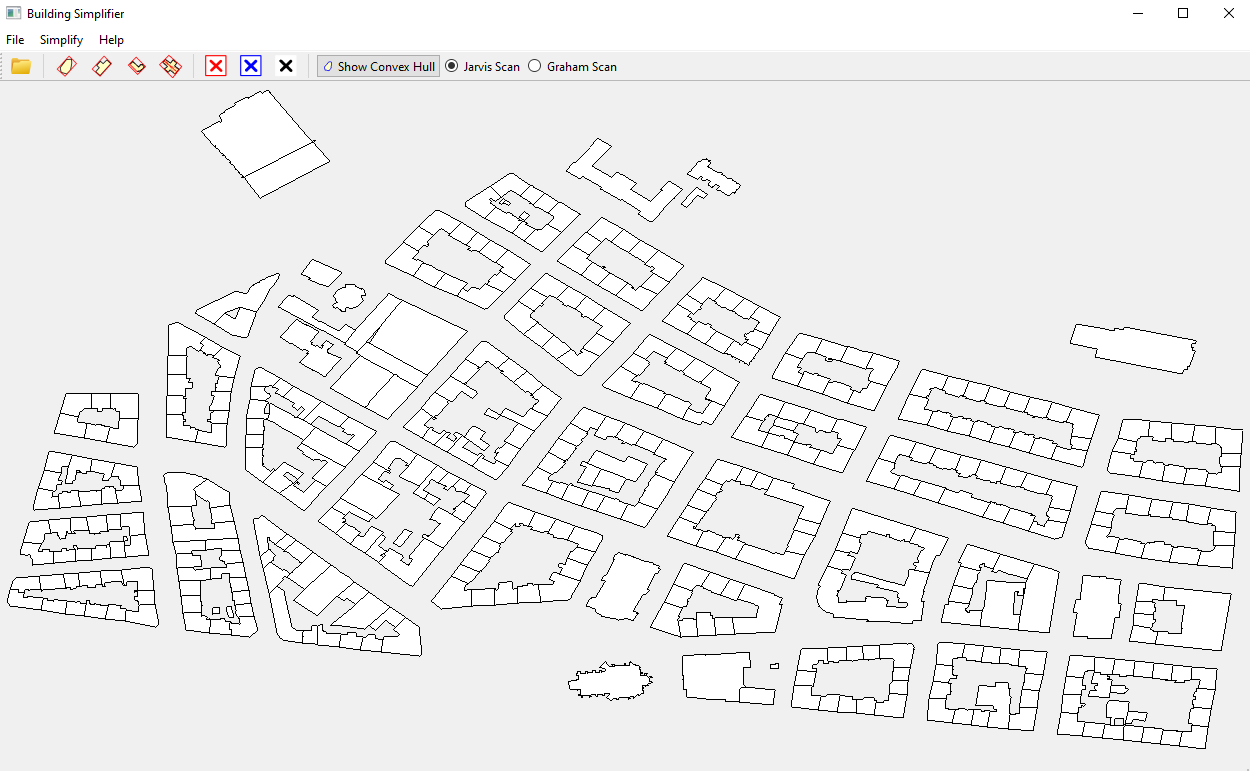
\includegraphics[width=14cm]{vinohrady_load.png}
    \caption{Ukázka načtených dat Vinohrad (vlastní zpracování).}
\end{figure}

\bigbreak

\section*{Aplikace}
\par Grafické rozhraní aplikace bylo vytvořeno v prostředí \verb|Qt Creator 9.0.1| a dále upravováno v prostředí programovacího jazyka \verb|Python 3.11|. Ovladatelnost a možnosti aplikace popisuje detailněji \emph{Obrázek 9}.

\begin{figure}[h]
\centering
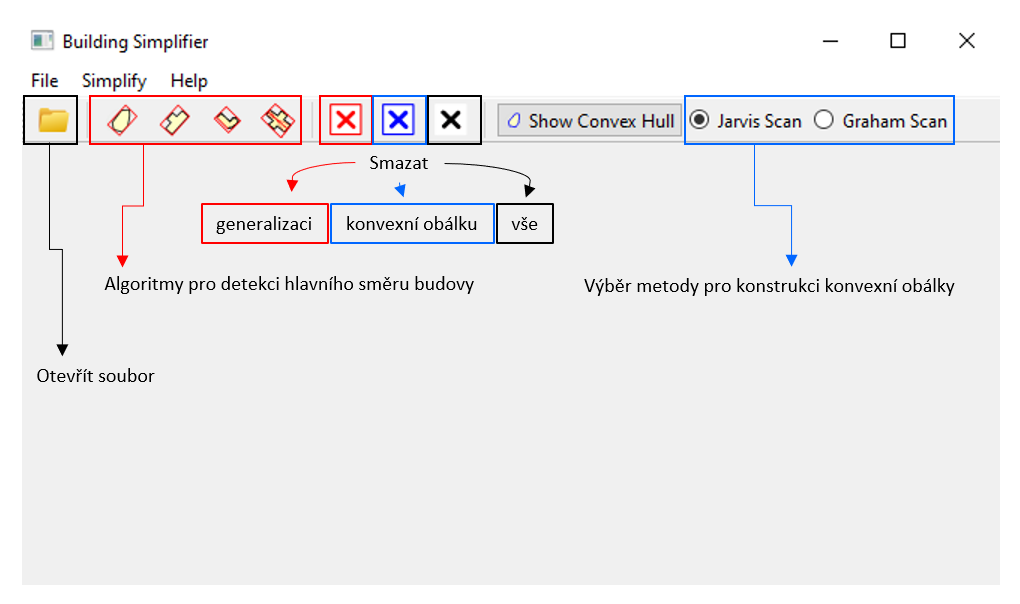
\includegraphics[width=15cm]{ukazka_graf_okno.png}
    \caption{Ukázka grafického okna aplikace s popisem funkcí (vlastní zpracování).}
\end{figure}

\par Uživatel má možnost na vstupních datech také zobrazit konvexní obálky jednotlivých polygonů (\emph{Obrázek 10}). Pokud je v datasetu nevalidní polygon (tj. např. polygon o dvou vrcholech nebo prázdný polygon), uživatel je upozorněn vyskakovacím oknem (\emph{Obrázek 11}) a tento prvek je vyloučen z dalšího zpracování.

\begin{figure}[h]
\centering
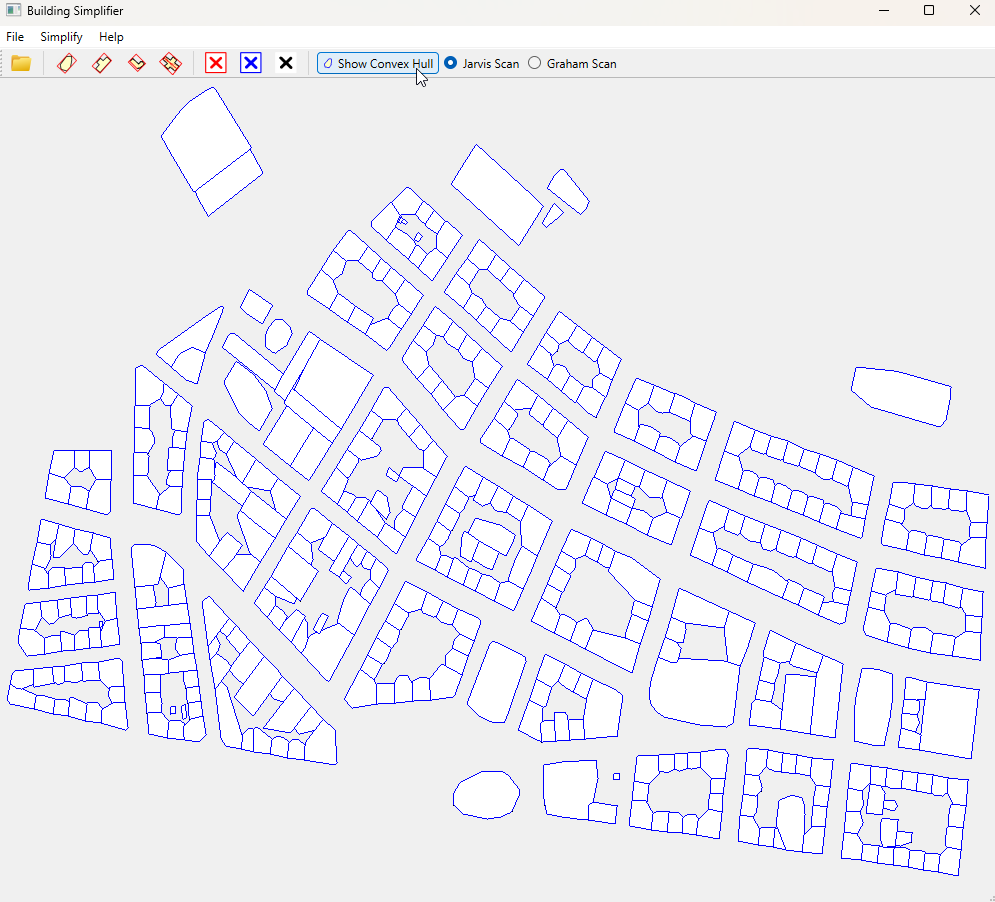
\includegraphics[width=8.5cm]{appch}
    \caption{Ukázka konvexních obálek vinohrad (vlastní zpracování).}
\end{figure}

\begin{figure}[h]
\centering
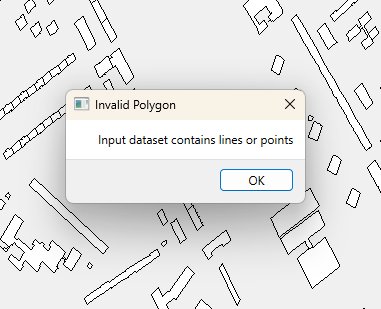
\includegraphics[width=9cm]{images/invalidinput.png}
    \caption{Ukázka vyskakovacího okna upozorňujícího na nevalidní polygon (vlastní zpracování).}
\end{figure}

\bigbreak

\section*{Třídy a metody}
\par Funkční chod aplikace si vyžaduje tři povinné skripty, v kterých jsou implementovány potřebné třídy a metody: \verb|mainform.py|, \verb|algorithms.py| a \verb|draw.py|.

\bigbreak

\par {\large\textbf{Třída MainForm} }
\par Třída MainForm ze souboru \verb|mainform.py| zabezpečuje inicializaci okna aplikace, vrchní lišty, panelu nástrojů, ikon a tlačítek. Zároveň přepojuje jednotlivé interaktivní položky okna s metodami, které vykonají specifické akce. Týkají se především otevření souboru, přepínání algoritmů apod. Část této třídy byla vygenerována v prostředí \verb|Qt Creator 9.0.1| (metody \verb|setupUi()| a \verb|translateUi()|). Níže jsou vyjmenovány nově implementované metody:

\begin{itemize}
    \item \verb|switchToJarvis()|
        \subitem{Nastaví algoritmus pro konstrukci konvexní obálky na \emph{Jarvis Scan}.}
    \item \verb|switchToGraham()|
        \subitem{Nastaví algoritmus pro konstrukci konvexní obálky na \emph{Graham Scan}.}
    \item \verb|constructCH()|
        \subitem{Provede konstrukci konvexní obálky. Metodě je předán seznam vstupních polygonů, na kterých se s využitím zvoleného algoritmu vytvoří jejich konvexní obálky. Pokud je nějaký z předaných polygonů nevalidní, konvexní obálka nebude vytvořena.}
    \item \verb|simplifyMAERClick()|
        \subitem{Provede generalizaci polygonu s využitím algoritmu \emph{Minimum Area Enclosing Rectangle}.}
    \item \verb|simplifyWallAverageClick()|
        \subitem{Provede generalizaci polygonu s využitím algoritmu \emph{Wall Average}.}
    \newpage
    \item \verb|simplifyLongestEdgeClick()|
        \subitem{Provede generalizaci polygonu s využitím algoritmu \emph{Longest Edge}.}
    \item \verb|simplifyWeightedBisectorClick()|
        \subitem{Provede generalizaci polygonu s využitím algoritmu \emph{Weighted Bisector}.}
    \item \verb|clearButton()|
        \subitem{Zavolá metodu \verb|clearCanvas()| z třídy \verb|Draw|, která vyprázdní okno.}
    \item \verb|clearERButton()|
        \subitem{Zavolá metodu \verb|clearERs()| z třídy \verb|Draw|, která smaže generalizované polygony.}
    \item \verb|clearCHButton()|
        \subitem{Zavolá metodu \verb|clearCHs()| z třídy \verb|Draw|, která smaže konvexní obálky.}
    \item \verb|exitClick()|
        \subitem{Ukončí aplikaci.}
    \item \verb|aboutClick()|
        \subitem{Otevře repozitář s aplikací v portálu \verb|GitHub|.}
    \item \verb|processFile()|
        \subitem{Zabezpečuje otevření souboru. Samotný soubor načte do proměnné pomocí metody \verb|openFile()| a následně zavolá metodu \verb|clearCanvas()| pro vyprázdnění okna. Pokud je vstupní \verb|JSON| nebo \verb|GeoJSON| nečitelný (např. nestandardní hierarchie položek v slovnících), uživatele na to upozorní vyskakovacím oknem.}
    \item \verb|openFile()|
        \subitem{Otevře \verb|JSON| nebo \verb|GeoJSON| soubor a načte ho do proměnné.}
\end{itemize}

\bigbreak

\par {\large\textbf{Třída Algorithms} }
\par V této třídě jsou obsaženy algoritmy, které byly popsány v kapitole \emph{Popis problému} věnované algoritmům pro konstrukci konvexní obálky a generalizace. Obsahuje tři skupiny metod: 

\begin{enumerate}
    \item Metody pro konstrukci konvexní obálky: Jarvis Scan, Graham Scan;
    \item Metody pro určení hlavního směru budovy: MAER, Wall Average, Longest Edge, Weighted Bisector;
    \item Pomocní metody pro zmíněné algoritmy (výpočet euklidovské vzdálenosti, nalezení min-max boxu, přizpůsobení velikosti min-max boxu, výpočet úhlů apod).
\end{enumerate}
\par První dvě skupiny již byly detailně popsány výše, třetí skupina obsahuje celkem 14 algoritmů uvedených níže. Jejich podrobnější popis se nachází uvnitř této třídy ve skriptu \verb|algorithms.py|.

\begin{itemize}
    \item \verb|get2LinesAngle(p1, p2, p3, p4)|
        \subitem{Vypočte úhel mezi dvěma vstupními liniemi.}
    \item \verb|getPolarAngle(p1, p2)|
        \subitem{Vypočte směrnici zadané linie.}
    \item \verb|vectorOrientation(p1, p2, p3)|
        \subitem{Udává pravotočivost, levotočivost nebo kolinearitu vektorů.}
    \item \verb|findPivot(pol)|
        \subitem{Nalezne pivota jako bod s minimálními souřadnicemi $x$ a $y$.}
    \item \verb|sortPoints(pol, q)|
        \subitem{Seřadí body vstupního polygonu vzestupně nejprv podle velikosti jejich polárního úhlu s pivotem $q$, pak podle jejich vzdálenosti od pivota $q$.}
    \item \verb|rotate(pol, sigma)|
        \subitem{Otočí polygon o úhel $\sigma$.}
    \item \verb|minMaxBox(pol)|
        \subitem{Vytvoří min-max box a vypočte jeho plochu.}
    \item \verb|computeArea(pol)|
        \subitem{Vypočte plochu libovolného konvexního útvaru.}
    \item \verb|resizeRectangle(er, pol)|
        \subitem{Změní velikost generalizované budovy vzhledem k její původní ploše.}
    \item \verb|checkValidity(pol)|
        \subitem{Zkontroluje, jestli je vstupní polygon validní.}
    \item \verb|euclidDistance(p1, p2)|
        \subitem{Vypočte euklidovskú vzdálenost mezi dvěma body.}
    \item \verb|findDiagonals(ch)|
        \subitem{Nalezne všechny uhlopříčky konvexní obálky a jejich velikosti.}
    \item \verb|intersectionTest(p1, p2, pol)|
        \subitem{Zjišťuje, jestli se vstupní úhlopříčka protíná s jednou z hran budovy.}
    \item \verb|setDiagonals(diagonals, pol)|
        \subitem{Vrátí dvě nejdelší uhlopříčky a jejich směrnice.}
\end{itemize}

\bigbreak

\par {\large\textbf{Třída Draw} }
\par Třída Draw ze souboru \verb|Draw.py| slouží pro inicializaci proměnných nesoucí prostorovou informaci, načítání a vykreslování geoprostorové informace. Při spuštění aplikace se inicializují proměnné pro seznam polygonů, seznam ohraničujících obdélníků (generalizovaných polygonů) a seznam konvexních obálek:

\begin{itemize}
  \item \verb|self.__polyg_list|,
  \item \verb|self.__er_list|,
  \item \verb|self.__ch_list|.
\end{itemize}

\par Třída Draw obsahuje následující metody:
\begin{itemize}
    \item \verb|paintEvent(e:QPaintEvent)|
        \subitem{Vykresluje objekty (bod a polygony) na plátno (Canvas).}
    \item \verb|clearCanvas()|
        \subitem{Smaže všechny objekty na plátně (Canvas).}
    \item \verb|clearERs()|
        \subitem{Vyprázdní seznam ohraničujících obdélníků.}
    \item \verb|clearCHs()|
        \subitem{Vyprázdní seznam konvexních obálek.}
    \item \verb|getPolygonList()|
        \subitem{Vrátí seznam vstupních polygonů.}
    \item \verb|getEnclosingRectangles(pols)|
        \subitem{Vrátí seznam ohraničujících obdélníků.}
    \item \verb|getConvexHulls(pols)|
        \subitem{Vrátí seznam konvexních obálek.}
    \item \verb|resizePolygons(xmin, ymin, xmax, ymax)|
        \subitem{Roztáhne vstupní data na plátno podle velikosti okna aplikace.}
    \item \verb|findBoundingPoints(p:QPointF, xmin, ymin, xmax, ymax)|
        \subitem{Nalezne minimální a maximální souřadnice pro ohraničení polygonu (tzv. bounding box).}
    \item \verb|loadData(data)|
        \subitem{Prochází slovník ze vstupního souboru \verb|JSON/GeoJSON| a načte geoprostorovou informaci.}
\end{itemize}